\section{Tests}
\subsection{Klebeversuch}


\begin{zebratabular}{p{4.5cm}p{\textwidth-3.6cm-0.7cm}}
	\rule{0pt}{11pt}\textit{Tester}           & Matteo Trachsel\\ 
	\rule{0pt}{11pt}\textit{Datum}:           & 06.03.2015\\
	\rule{0pt}{11pt}\textit{Beschreibung}:    & Das Ziel dieses Testes bestand darin, den 
												gekauften Kleber UHU Hart auf seine Klebekraft und auf sein Erscheinungsbild zu testen.\\
	\rule{0pt}{11pt}\textit{Akteure}:         & Acrylglas \\
	\rule{0pt}{11pt}\textit{Bedingung}:       & Für den Test werden verschiedene Acrylglas-Stücke zusammengeklebt.
	Hierfür wird der Kleber wie auf der Gebrauchsanweisung auf zwei Verfahren getestet. 
	Im ersten Versuch wird der UHU Kleber aufgetragen und die zwei Platten zusammengeklebt. 
	Im zweiten Versuch wird der Kleber zuerst auf die Acrylglasstücke aufgetragen und 
	gewartet bis er angetrocknet ist, danach noch einmal eine Schicht vom Kleber aufgetragen 
	und zusammengefügt.\\
	\rule{0pt}{11pt}\textit{Erwartete Fehlermeldung}:          & keine \\
	\rule{0pt}{11pt}\textit{Vorgehen}:        & Kleber auf Acrylglas, zusammenhalten \\
	\rule{0pt}{11pt}\textit{Erwartetes Ergebnis}: & Mit dem Versuch konnte gezeigt werden, dass der Kleber sicher glasklar bleibt. Weiter 
	ist die erwünschte Klebekraft bestätigt worden. Beim zweiten Versuch, wo zuerst der 
	Kleber etwas angetrocknet wurde, ist eine deutlich schlechtere Klebekraft festgestellt 
	worden. Dadurch wird der Kleber immer sofort aufgeklebt.\\
	\rule{0pt}{11pt}\textit{Eingetretenes Ergebnis}: & Alles IO.\\
	\rule{0pt}{11pt}\textit{Test bestanden?}:     & Ja \\
\end{zebratabular}  


\begin{figure}[h!]
	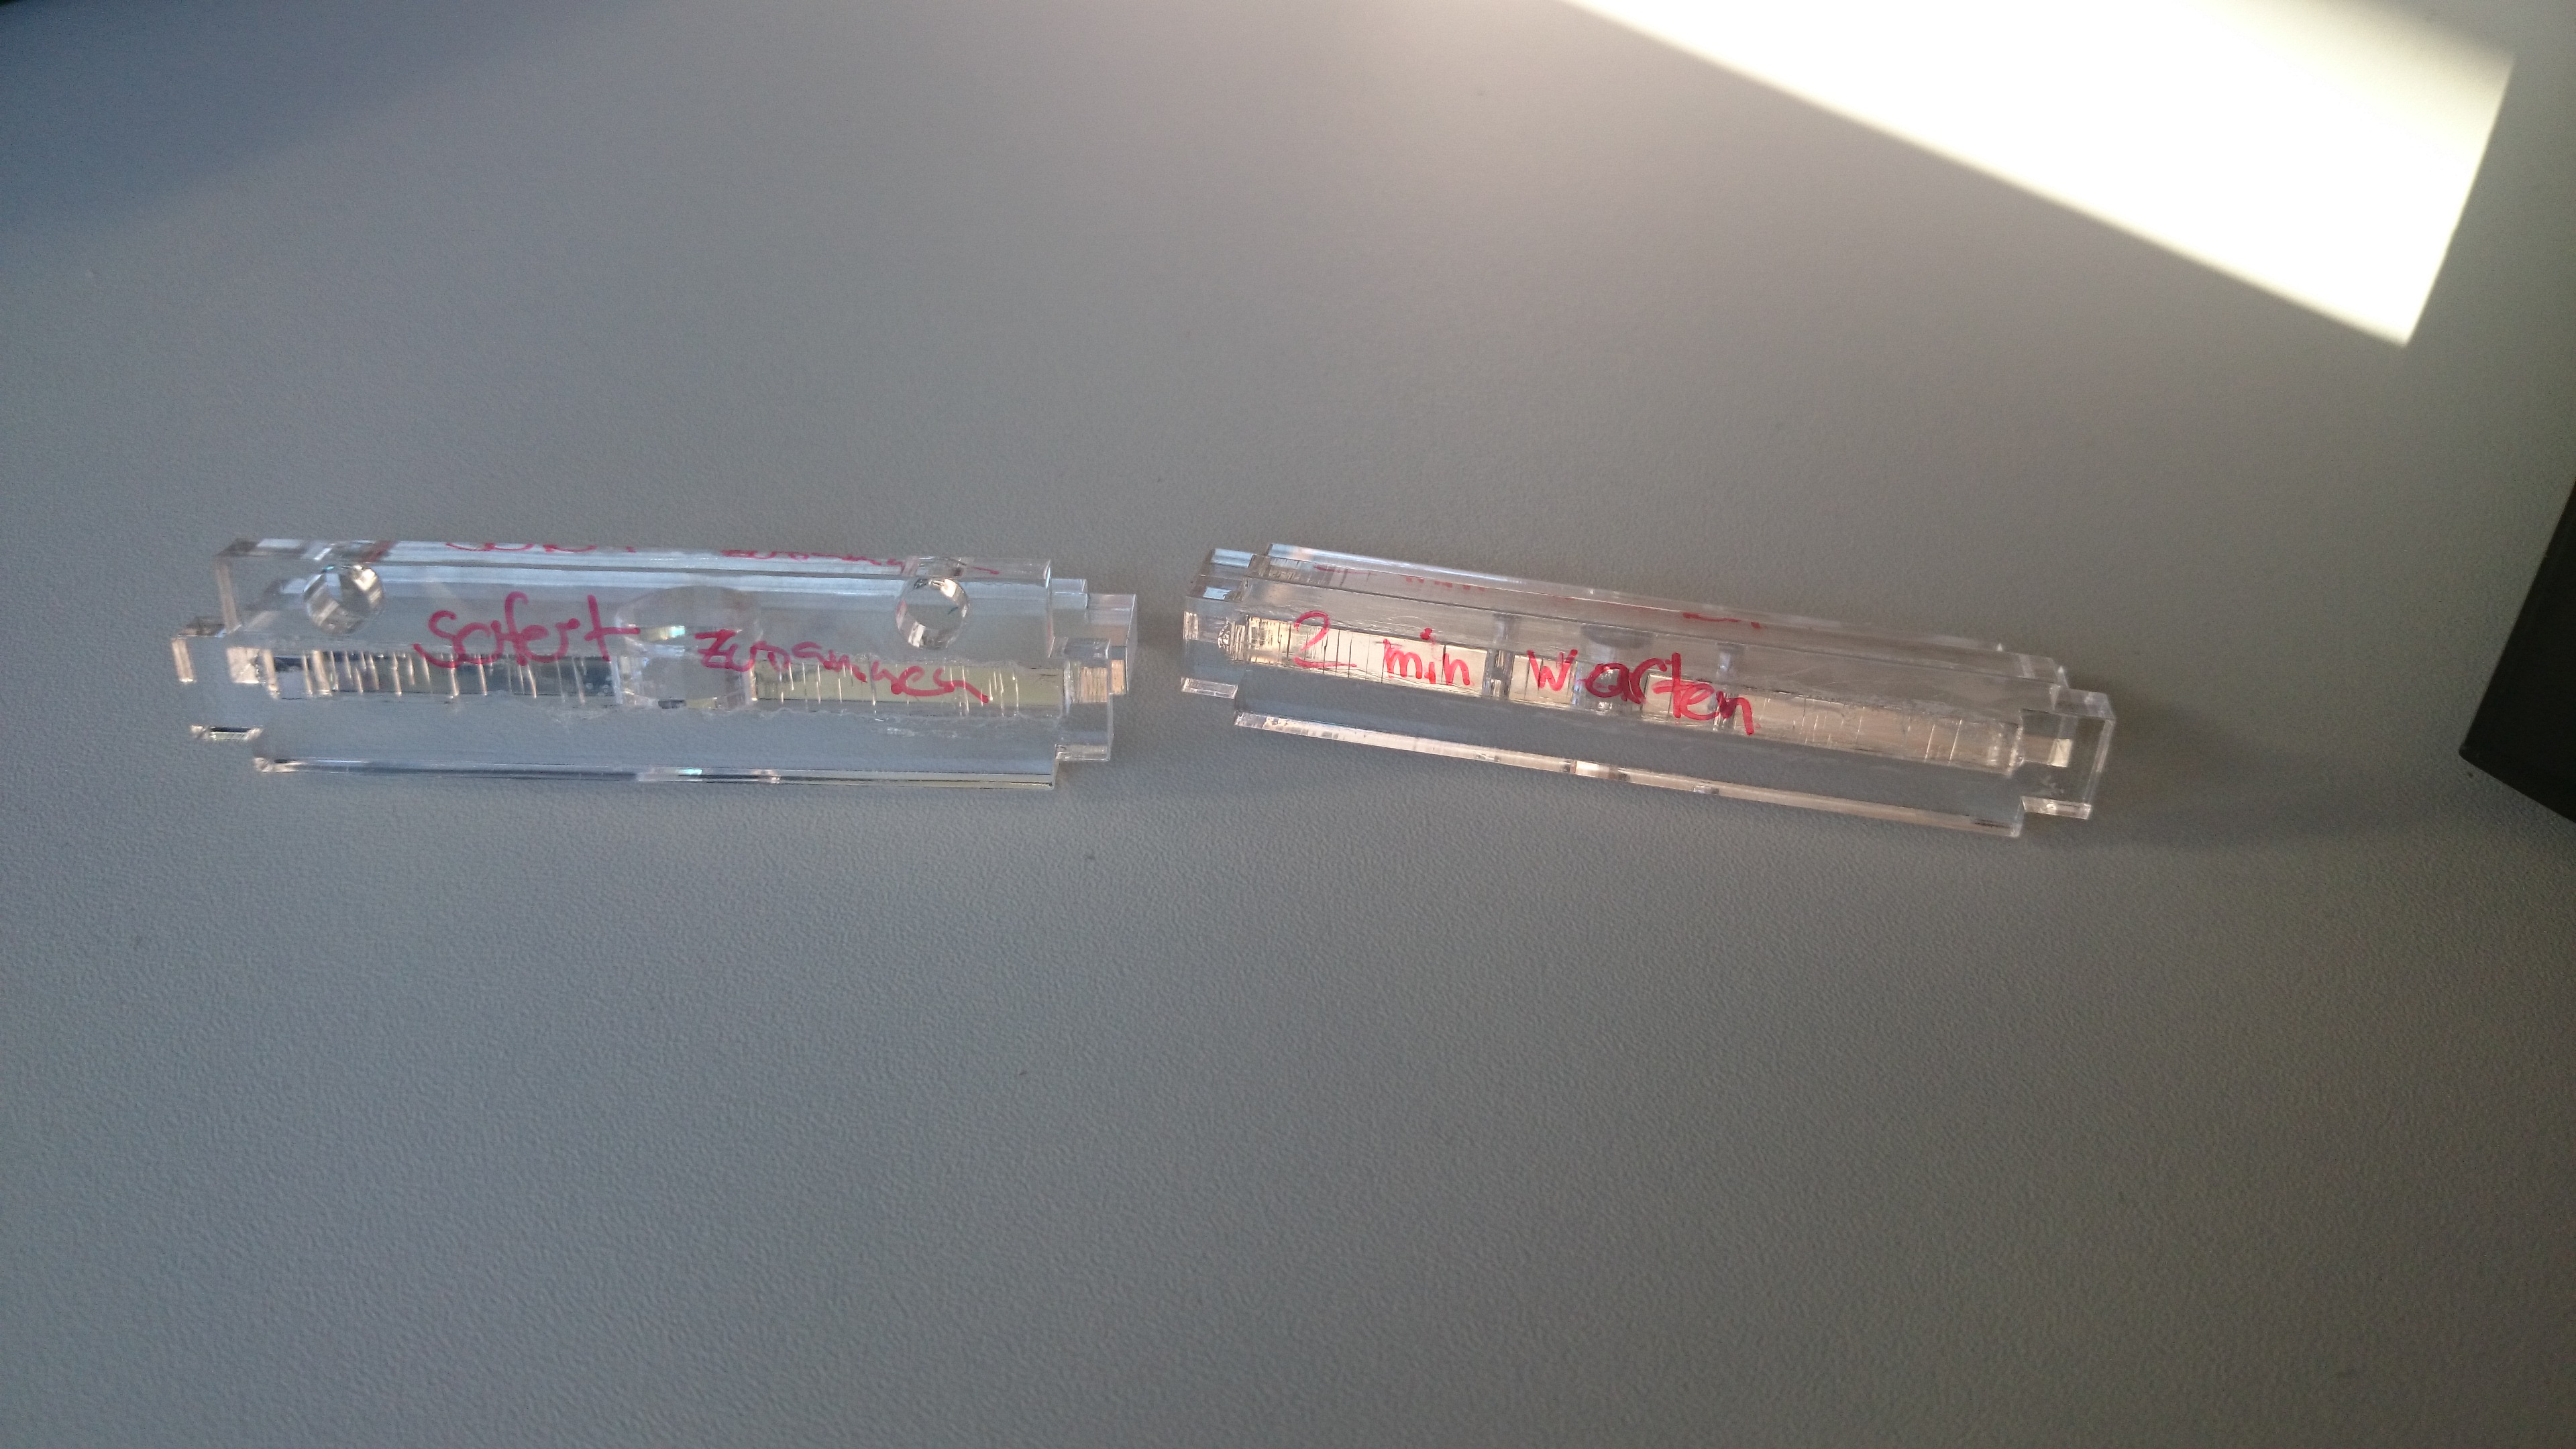
\includegraphics[width=0.7\textwidth,clip,trim=0cm 0cm 0cm 0cm]
	{Testberichte/Klebeversuch.jpg}
	\centering
	\caption{Klebeversuch mit UHU Kleber} 
	\label{abb:Klebeversuch}
\end{figure}